\section{Appendix C: Public Disseminations} 
\begin{flushright}
    \textit{''T'as pas de doutes ? Moi j'en ai,\\
    (...)\\
    Je sais pas ce que c'est, \\
    C'est l'Inconnu.''}\\
    Cadillac \& KingJu, Egoslave, 2018
\end{flushright}
\label{appendix_public_articles}

\subsection{Rationale and open-access}

There are several reasons why public research should be made publicly available. On the professional side, having any scientist able to access in-depth research, and not just the research manuscript, vastly improves the quality of any scientific field as a whole. On the ethical side, having an open policy on research effectively deprives predatory publishing companies of their revenues, vastly improving the quality of life of all scientists~\cite{smith2023imaging}. For these two reasons, when possible (i.e. not under embargo for a publication in production), the code that has been written during this thesis and its associated data is available online for open access:
\begin{itemize}
    \item Related to this entire manuscript: \\
    Code: \href{https://github.com/hugoladret/PhD_manuscript}{\url{https://github.com/hugoladret/PhD_manuscript}}
    \item Related to Chapter's 3 article on Convolutional Sparse Coding: \\
    Data: \href{https://doi.org/10.6084/m9.figshare.24167265}{\url{https://doi.org/10.6084/m9.figshare.24167265}} \\
    Code: \href{https://github.com/hugoladret/epistemic_CSC}{\url{https://github.com/hugoladret/epistemic_CSC}}
    \item Related to Chapter's 4 article on Cortical Recurrence in \gls{V1}: \\
    Data: \href{https://doi.org/10.6084/m9.figshare.23366588.v2}{\url{https://doi.org/10.6084/m9.figshare.23366588.v2}} \\
    Code: \href{https://github.com/hugoladret/variance-processing-V1}{\url{https://github.com/hugoladret/variance-processing-V1}}
\end{itemize}

Finally, on the logical side, since this research is paid by taxpayer's money, it should be made available to the taxpayer. Taxes are not just paid by researchers (thankfully for us), but by people with a heterogeneous scientific formation, and as such, it is crucial that scientific productions end up being formatted in such a way that anyone might benefit from them. In that regard, this thesis also includes two public dissemination articles in French, with English translation provided here after each article.


\subsection{Article 1 (Sciences et Avenir)}
The first public dissemination article is based on an interview by Alice Carliez, derived from our article \fullcite{ladret2023cortical}, for the French journal \textit{"Sciences et Avenir"}.

% avant d'intégrer un article dans votre thèse, consulter http://www.sherpa.ac.uk/romeo/ si vous souhaitez diffuser sur internet
\includepdfset{pagecommand=\thispagestyle{scrheadings}} % ajoute la numérotation continue des pages aux fichiers pdf importés
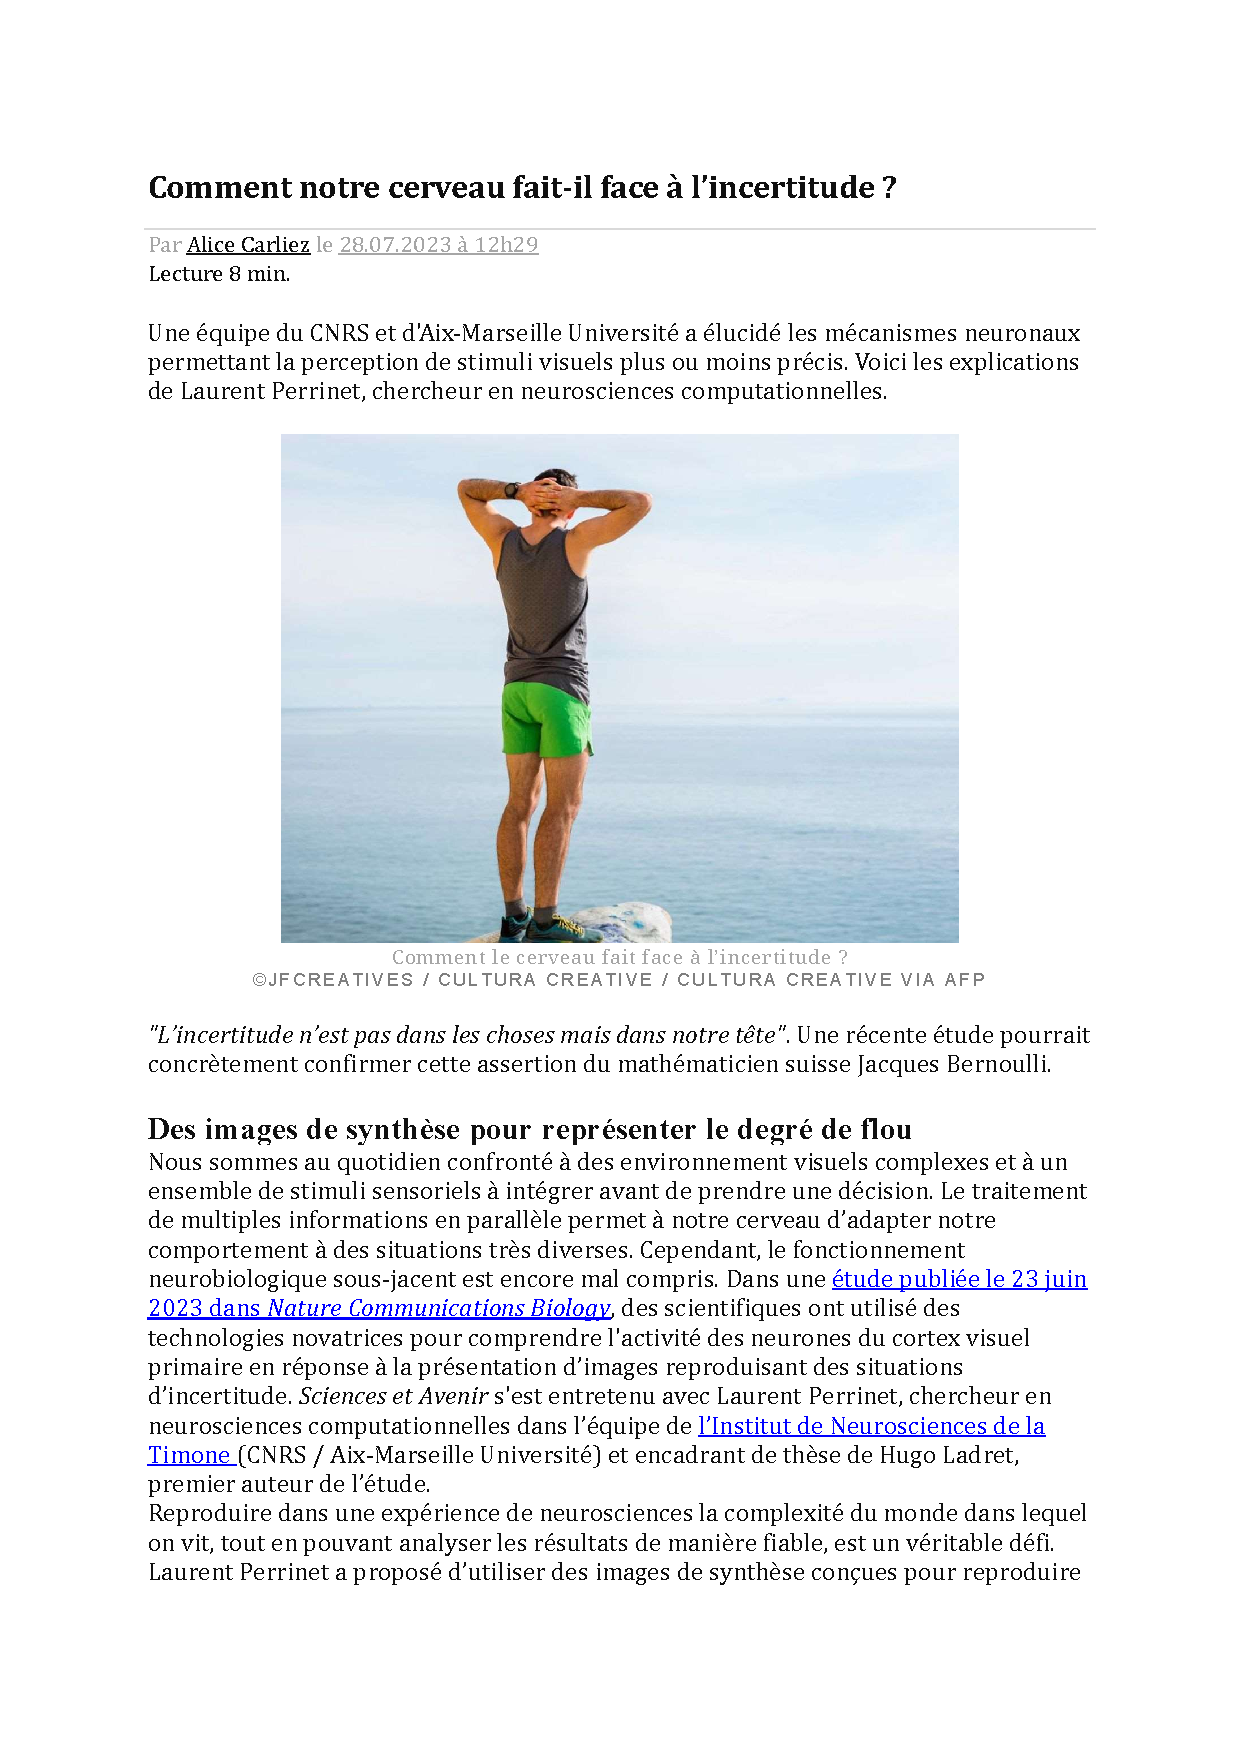
\includepdf[scale=0.86,pages=-]{tex_append/sciences_et_avenir.pdf} % 'scale' ajuste la taille du pdf, vous pouvez affiner en fonction des marges
\clearpage
\textbf{English translation}:

\textbf{How does our brain deal with uncertainty?}

A team from CNRS and Aix-Marseille University has elucidated the neural mechanisms that enable the perception of more or less precise visual stimuli. Here are the explanations by Laurent Perrinet, a researcher in computational neuroscience.

Every day, we are confronted with complex visual environments and a range of sensory stimuli to integrate before making a decision. Processing multiple pieces of information in parallel enables our brain to adapt to a wide variety of situations. However, the underlying process is still poorly understood. In a study published in June 23 2023 in Nature Communications Biology, scientists have used innovative technologies to understand the activity of neurons in the primary visual cortex cortex in response to the presentation of images reproducing situations of uncertainty. Sciences et Avenir spoke to Laurent Perrinet, a computational neuroscientist computational neuroscience researcher in the team at the Institut de Neurosciences de la Timone (CNRS / Aix-Marseille University) and Hugo Ladret's thesis supervisor, first author of the study.

Reproducing the complexity of the world in which we live in a neuroscience experiment, while still being able to analyze the results reliably, is a real challenge. Laurent Perrinet has proposed the use of computer-generated images designed to reproduce an uncertain visual context. Like the textures used in two-dimensional video games, these images represent elongated patterns, oriented more or less in the same direction. When all the patterns have the same orientation, it's easy to guess which is their orientation. On the other hand, when many different orientations are present, visual information is much less clear. These textures allow us to reproduce the natural images we are confronted with. While we can sometimes identify an object very well, other perceived elements appear more blurred and uncertain. When it comes to using textures, the problem is the same: sometimes there are lines whose orientation is easily identifiable, and sometimes there are scattered dots whose organization is imprecise.

The use of these textures is innovative. Traditionally, neuroscience researchers have used rather isolated shapes to stimulate visual areas: a rectangle, a dot, a moving line. "The fact of having such simple images is useful for analysis. But these isolated shapes are not 'ecological'. So we have to find another way of reproducing our more complex world. Especially as the brain is adapted to perceiving very rich images," explains Laurent Perrinet to Sciences et Avenir.

The brain is designed to perceive both precise objects: their shape, direction, orientation, contours, colors... But also to understand more uncertain situations, in order to interpret the disorder and chaos that confuse our anticipations. Computer-generated textures are a way of reproducing the natural images we are confronted with. Starting from a mathematical theoretical intuition, Laurent Perrinet's team first asked themselves how the brain can leave room for uncertainty.

\textbf{Some neurons are specialized in uncertainty}
Scientists recorded the activity of 249 neurons in anesthetized cats. They observed the response of neurons in the primary visual area to the presentation of more or less blurred images. They found that there were two types of neuronal response to uncertainty. Vulnerable" neurons respond only to a certain orientation. They are highly sensitive and vulnerable to large degrees of vagueness. And "resistant" neurons, which respond to visual stimuli despite the lack of precision of the visual information. Even when animals are presented with textures that are not well-defined, i.e. whose orientation is indistinguishable, these neurons continue to respond.
"If a person is shown textures that are among the most imprecise within the texture range, from 30° of imprecision, people get confused and can't find the orientation of the texture lines. But there are still neurons that respond precisely", explains Laurent Perrinet.

\textbf{"I bet you that in the brain, there is a representation of the blur"}
The researchers therefore wanted to go further than simply observing neuron activity. They looked to see if, from this activity, it was possible to reconstruct the type of texture presented in the first place. They achieved this deciphering through machine learning processes similar to those used in Deep Learning.   "It all started from discussions between us and a bet between the scientists ''I bet you that in the brain, there is a representation of the blur'", says the researcher.The experiment is conducted in such a way as to understand the encoding of visual information, based on the activity of neurons, thanks to a "decoding" stage.Three stages can be defined:
\begin{itemize}
    \item Encoding: the luminous information caused by the image is captured by the eyes.
    \item Coding: the recording by the neuronal activity that perceive this encoding.
    \item Decoding: the translation of the neuronal activity via a Machine Learning algorithm, to retrieve the orientation of the lines on the images presented to the eyes.
\end{itemize}
To the surprise of the scientists, this decoding step works extremely well: the decoding software developed here can retrieve the orientation of the lines of the texture with great performance. Furthermore, when the image was blurry, they observed that the decoding was also more blurry, and appeared with a delay. The results confirm that the population of the neurons in the primary visual cortex can not only retrieve the orientation of an object, but also interpret whether that information is precise or not. The brain is capable of representing imprecise visual stimuli, and distinguish whether one information is precise or not. "For a neural network, it is important to decipher both the nature and the precision of visual information, to be able to make a decision. The brain works tirelessly, with neurons working together to exchange and integrate packets of information, which can take time before reaching a consensus. Hence, the importance of uncertainty to weigh more or less some information, to save time and facilitate decision-making", explains Laurent Perrinet.

\textbf{The brain, a predictive machine}.
"The brain should not be considered as a computer, but as a prediction machine. A set of cells that want what's best for us and work for our survival, making decisions that can be understood using a probabilistic model," illustrates Laurent Perrinet. In his view, it would be a mistake to draw an analogy between brain function and that of a sequentially operating computer. The theory of the "predictive brain" proposes that neuronal cells function continuously and in groups, to integrate the multiplicity of sensory information perceived, in order to make a decision. In order for this decision to be taken as smoothly as possible, despite the imprecision associated with our senses, it would be necessary for neurons to make predictions.

"We're currently seeing a technological revolution in Machine Learning on the use of deep networks, ChatGPT etc.... These technologies are based on neural networks which enable extraordinary performance, but which are not yet equal to that of the brain. The latter consumes 5 to 20 Watts. A current GPU (Graphical Processing Unit, an alternative architecture to the processors commonly used in Deep Learning, editor's note) is 600 Watts, and the one that beat the Go world champion is 20 Megawatts! continues the researcher. It's marvellous that we can now use these deep learning intelligences in healthcare or for so many other activities. But I think we have to bear in mind that these technologies are still very sensitive to errors. This doesn't seem to be a problem if a technology's task is simply to distinguish a cat from a dog. On the other hand, it could be dangerous if AIs are used in medical imaging, where variability in the data received could influence the veracity of the diagnosis. If we want AIs to have the efficiency of the brain, we would have to include in each node of this network, in addition to the values, their uncertainty. Instead of using current networks that operate in an analogical way, we could implement a probabilistic operation". The researcher wants to give uncertainty a place. Just as our brains do.



\clearpage



\subsection{Article 2 (Cerveau et Psycho)}
The second public dissemination article was written by Laurent Perrinet and myself, based on our article \fullcite{ladret2023cortical}, to be published in the French journal \textit{"Cerveau et Psycho"}. Compared to the first dissemination article, this one dives (slightly) more into the philosophical implications of processing uncertainty, as well as providing more common sense into the notion of uncertainty in natural images.

% avant d'intégrer un article dans votre thèse, consulter http://www.sherpa.ac.uk/romeo/ si vous souhaitez diffuser sur internet
\includepdfset{pagecommand=\thispagestyle{scrheadings}} % ajoute la numérotation continue des pages aux fichiers pdf importés
\includepdf[scale=0.88,pages=-]{tex_append/cerveau_et_psycho.pdf} % 'scale' ajuste la taille du pdf, vous pouvez affiner en fonction des marges
\clearpage
\textbf{English translation}:

\textbf{A brain that guesses is a brain that doubts}

\textbf{Introduction}

If you were asked which of these two portraits gives the most faithful rendering of a facial expression, you would probably reply that it is the iconic Mona Lisa. However, if you were now asked which of these two faces reveals emotion more clearly and precisely, you would probably find it easier to read the laughing thoughts rendered in Antonello da Messina's portrait. It seems, then, that even if you perceive the Mona Lisa as more "alive", it doesn't make her any more comprehensible to you. Intriguing, isn't it? Although both figures emanate the same air of mystery, there is something about the Mona Lisa that gives it a bewitching singularity.

In the light of modern scientific analysis, we now have a better understanding of why the portrait of Mona Lisa appears so authentic and so mysterious. The work's legendary ambivalence allows the Mona Lisa's gaze to follow the viewer, and her smile to appear to change depending on the angle from which she is viewed. Da Vinci, a keen observer of the world around him, masterfully used realistic techniques to bring to life an image that, while static, evokes a dynamic presence comparable to those we encounter in our everyday lives. The visual ambiguity induced by the observation of the Mona Lisa, a central aspect of its mystery, is reminiscent of the way sunlight finds its way through foliage in a forest, playing subtly with shadows to create an atmosphere that is both lively and enigmatic.

The enigmatic realism of the portrait of the Mona Lisa is down to the talent of its creator. Da Vinci was an undisputed master of sfumato, an arduous artistic technique used to soften the contours of a painting for a more natural, realistic effect. This is a fine example of his multidisciplinary genius, for da Vinci, with only the knowledge of his time, seemed to anticipate certain advances in modern science on natural images. Indeed, we now know that our brains are finely tuned to analyse the visual world around us from every angle. In particular, a system of brain areas processes the information coming from the retina, starting by breaking down the world around us into small, oriented and subtle outline elements, meticulously reproduced in the sfumato of the Mona Lisa. These contours form the framework of our visual perception, from which our brain sketches an image of the luminous world around us.

\textbf{Analysis of Natural Images}

Like the enigmatic smile of the Mona Lisa, natural images are themselves imbued with uncertainty and complexity. Take, for example, the glaring difference between the decompositions of orientations that form the contours of a tree and those that draw a boat, as depicted in the figure above. The different uncertainties of these contours measure fundamentally distinct degrees of ambiguity and perfectly illustrate the variety inherent in our visual environment.

In a modern context, this is all the more important. Imagine yourself as a pedestrian, in the middle of a city, about to cross the road at a crossing without traffic lights. You stare at the driver of the nearest car, trying to read his intentions on his face. Should you trust his staring eyes? Or take into account the uncertainty of his car, which has slowed down but not quite braked? Should you expect a hand gesture to resolve this uncertainty? So many visual variables to consider in order to reduce the uncertainty as to whether the driver is going to stop, while hoping that his face is less mysterious than the Mona Lisa.

\textbf{Brain that guesses}

So there's no doubt that uncertainty is a fundamental issue in psychology. But what about the 'brain' itself? A recent study we conducted at the Institut des Neurosciences de la Timone (Aix-Marseille University; CNRS) in collaboration with the University of Montreal sheds some light on this subject.

By observing neurons involved in vision, and in particular in the representation of oriented contours, we have identified that different neurons do not all have the same sensitivity to uncertainty. As a result, it is possible to 'read' the uncertainty contained in an image from the activity of neuronal populations. This 'reading', which we have done with Artificial Intelligence, could also be done by the brain using its specialized neural networks. This would explain why our perception is so sensitive to uncertainty, and how uncertainty could control our behaviour. Despite the fact that these neurons sensitive to uncertainty only represent a third of the total population, they nevertheless play a crucial role in providing the entire neural system with data that improves signal processing, by adding an assessment of its probability and degree of confidence.

Although this discovery is captivating, it is hardly surprising. The brain has mastered the art of navigating through an ocean of fragmented and ambiguous information to forge, through our perception, a coherent vision of reality. We can easily reconstruct images even when they are partially obscured by shadows or distortions. In rare cases, such as da Vinci's masterpiece, we find ourselves faced with a veritable labyrinth of ambiguities where several interpretations of a stimulus are possible. So which should we choose? The Mona Lisa's enigmatic smile or her penetrating gaze that seems to follow us? The uncertainty of these clues is crucial in piecing together the fragments of our perception. The brain, in this sense, acts like a sculptor, modelling our reality from hypotheses based on probabilities, in accordance with the etymology of the term "fiction", which implies modelling or shaping. All the more so because this process is dynamic and incorporates various sources of information (vision, proprioception, sound, etc.) to achieve a unified perception. This applies even in complex situations, such as distinguishing several voices in the din of a dinner party.

This paradigm has important implications for understanding various neuropsychological substrates. Recent theories confirmed by our results suggest that neurons communicate with each other to exchange information about the uncertainty of a situation. For example, different balances in this integration mechanism could explain certain conditions such as schizophrenia, where the perception of reality can be modified by reduced beliefs about the external world, which is considered too uncertain. Conversely, the privileged processing of sensory information observed in the autistic spectrum could be interpreted by a different balance between a mind that is certain of its perceptions in a world that is still full of uncertainties.

\textbf{Brain that doubts}

Our knowledge and uncertainties - be they scientific, cultural or other - shape our lives and our societies in many ways: they influence our purchasing behaviour, guide our holiday choices, and even have an impact on issues as global as climate change. In this last area, each of us plays a role, often without fully realizing it. Acknowledging the limits of our knowledge and admitting that we don't have all the answers means we can better weigh up the pieces of the decision-making jigsaw in which we engage on a daily basis. In this way, becoming aware of the mechanisms of our cognition, which is based on approximations and uncertainties rather than on rigid, infallible logic, can help us to make more enlightened and more humane choices for society. Our world is gradually being governed more and more by artificial intelligence algorithms that reinforce our cognitive biases and compartmentalize our opinions into bubbles impervious to uncertainty. The transition from \textit{Homo Sapiens}, convinced of his certainties, to \textit{Homo Dubitans}, gifted with the rational doubt that reflects his natural intelligence, seems not only desirable but necessary if we are to meet the future challenges facing humanity.